\documentclass{beamer}
\usepackage[american]{babel}
\usepackage{subcaption}
\usepackage{multirow}
\usetheme{Frankfurt}
\usepackage{multicol}
\usepackage{graphicx}
\newcommand{\bit}[1]{\ensuremath{\textbf{\textit{#1}}}}
\newcommand{\dsp}{\ensuremath{\displaystyle}}
\setbeamerfont{page number in head/foot}{size=\large}
\setbeamertemplate{navigation symbols}{}
\setbeamertemplate{footline}[frame number]

%\usepackage{caption}
%\captionsetup{justification=raggedleft, singlelinecheck=false}

\title{Non-linear self-interference cancellation on base of mixed Newton method}
%\subtitle{Модуль адаптивной компенсации паразитных помех в приёмном тракте мобильного терминала}

\author[Degtyarev Alexander]{Graduate student Degtyarev Alexander Andreevich\\ 
\small Supervisor: DSc, Dvorkovich Alexander Viktorovich \\
\small Scientific consultant:  PhD, Bakhurin Sergey Alexeyevich}
\institute{MIPT \\
Department of Multimedia Technologies and Telecommunications
}
\date{2023-11-23}
\begin{document}
\begin{frame}[plain]
\titlepage
\end{frame}


\begin{frame}
\frametitle{Contents}
\tableofcontents
\end{frame}


\section{Introduction}
\subsection{In-band full-duplex systems idea}

\begin{frame}
\frametitle{Topic relevance}
Requirements:
\begin{itemize}
\item Effective resources arrangement among users
\item Networks with high reliability, low latency, and high data rates
\end{itemize}
In-band full-duplex technology (IBFD) provides:
\begin{itemize}
	\item Efficient exploitation of the spectrum, by frequency bandwidth sharing between transmitter and receiver
\end{itemize}
\textbf{IBFD systems suffer from undesired self-interference at the receivers path}
\end{frame}

\subsection{Self-interference cancellation issue}
\begin{frame}
	\frametitle{Self-interference cancellation (SIC) issue}
	\begin{figure}[htbp]
		\centering
		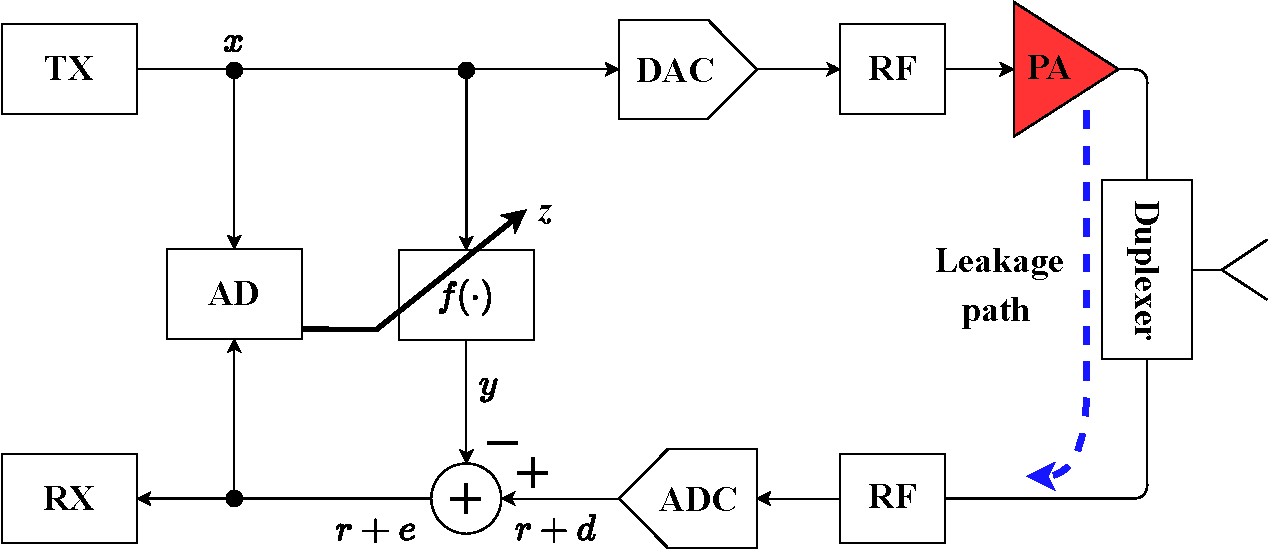
\includegraphics[scale=0.33]{../figures/ident_problem/ident_problem.pdf}
		\caption{Full-duplex transceiver simplified scheme \{Degtyarev A., draw.io\}}
%		\caption*{Degtyarev Alexander, draw.io}
	\end{figure}
	\begin{itemize}
		\item RF-chipset integral implementation and isolation issues $\rightarrow$ TX leakage to RX
		\item TX signal $\bit{x}$ is distorted in non-linear components (PA, Duplexer) and TX-RX leakage path
		\item SIC is an interference identification task:
		\begin{equation}
			\dsp\mathcal{J}(\bit{h})=\mathbb{E}\Big(|\bit{r}+\bit{d}-\bit{y}|\Big)^2\rightarrow\min_{\bit{h}},
		\end{equation}
	\end{itemize}
\end{frame}

\section{Adaptive compensation of self-interference}
\subsection{Non-linear interference model}
\begin{frame}
	\frametitle{Non-linear interference model}
	\begin{figure}[htbp]
		\centering
		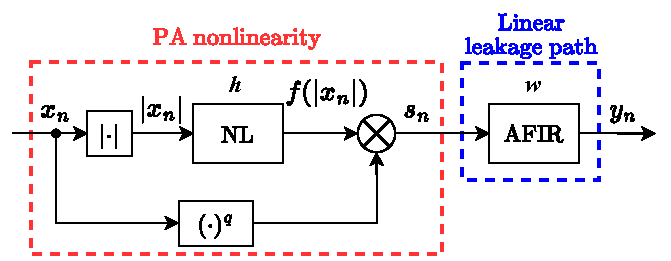
\includegraphics[scale=0.7]{../figures/hammerstein/hammerstein.pdf}
		\caption{Hammerstein model \{Degtyarev A., draw.io\}}
	\end{figure}
	\begin{itemize}
		\item Behavioral Hammerstein model describes interference creation physical process $\rightarrow$ low-complexity
		\item Hammerstein model output sample:
	\begin{equation}
		y_n=\sum_{m=-D}^{D}w_m\sum_{k=0}^{P-1}h_k x_{n-m}NL(|x_{n-m}|),
		\label{hammerstein_output}
	\end{equation}
	$w_m\in\mathbb{C}, h_k\in\mathbb{C}$ -- FIR and NL adaptive parameters.
	\end{itemize}
\end{frame}

\subsection{Mixed Newton method}
\begin{frame}
	\frametitle{Introduction to mixed Newton method}
	\begin{itemize}
		\item Mixed Newton method (MNM) -- second order method:
		\begin{equation}
			\bit{z}_{k+1}=\bit{z}_{k}-\mu_k(\bit{H}_{\bit{z}, \bit{z}^*}J)^{-1}(D_{\bit{z}^*}J)^T,
		\end{equation}
		$\bit{z}^T=(\bit{h}^T \bit{w}^T)\in\mathbb{C}^{1\times K}$ -- parameter vector, $J=\bit{e}^H\bit{e}$ -- MSE.
		\item For holomorphic error $\bit{e}=\bit{d}-\bit{y}$: $D_{\bit{z}^*}\bit{e}=\bit{0}$, mixed hessian and gradient are expressed through jacobian:
		\begin{equation}
			\bit{H}_{\bit{z}, \bit{z}^*}J=(D_{\bit{z}}\bit{y})^HD_{\bit{z}}\bit{y};
			\text{			}
			(D_{\bit{z}^*}J)^T=(D_{\bit{z}}\bit{y})^H\bit{e}
		\end{equation}
		\item For holomorphic error $\bit{e}$ method repulses from saddle points.
		\item Computational complexity defined by hessian calculation and inversion:
		\begin{equation}
			\chi_{\text{MNM}}=\mathcal{O}(K^3+K^2N)
		\end{equation}
	\end{itemize}
\end{frame}

\subsection{Experimental setup}
\begin{frame}
	\frametitle{Experimental setup}
	\begin{figure}[htbp]
		\centering
		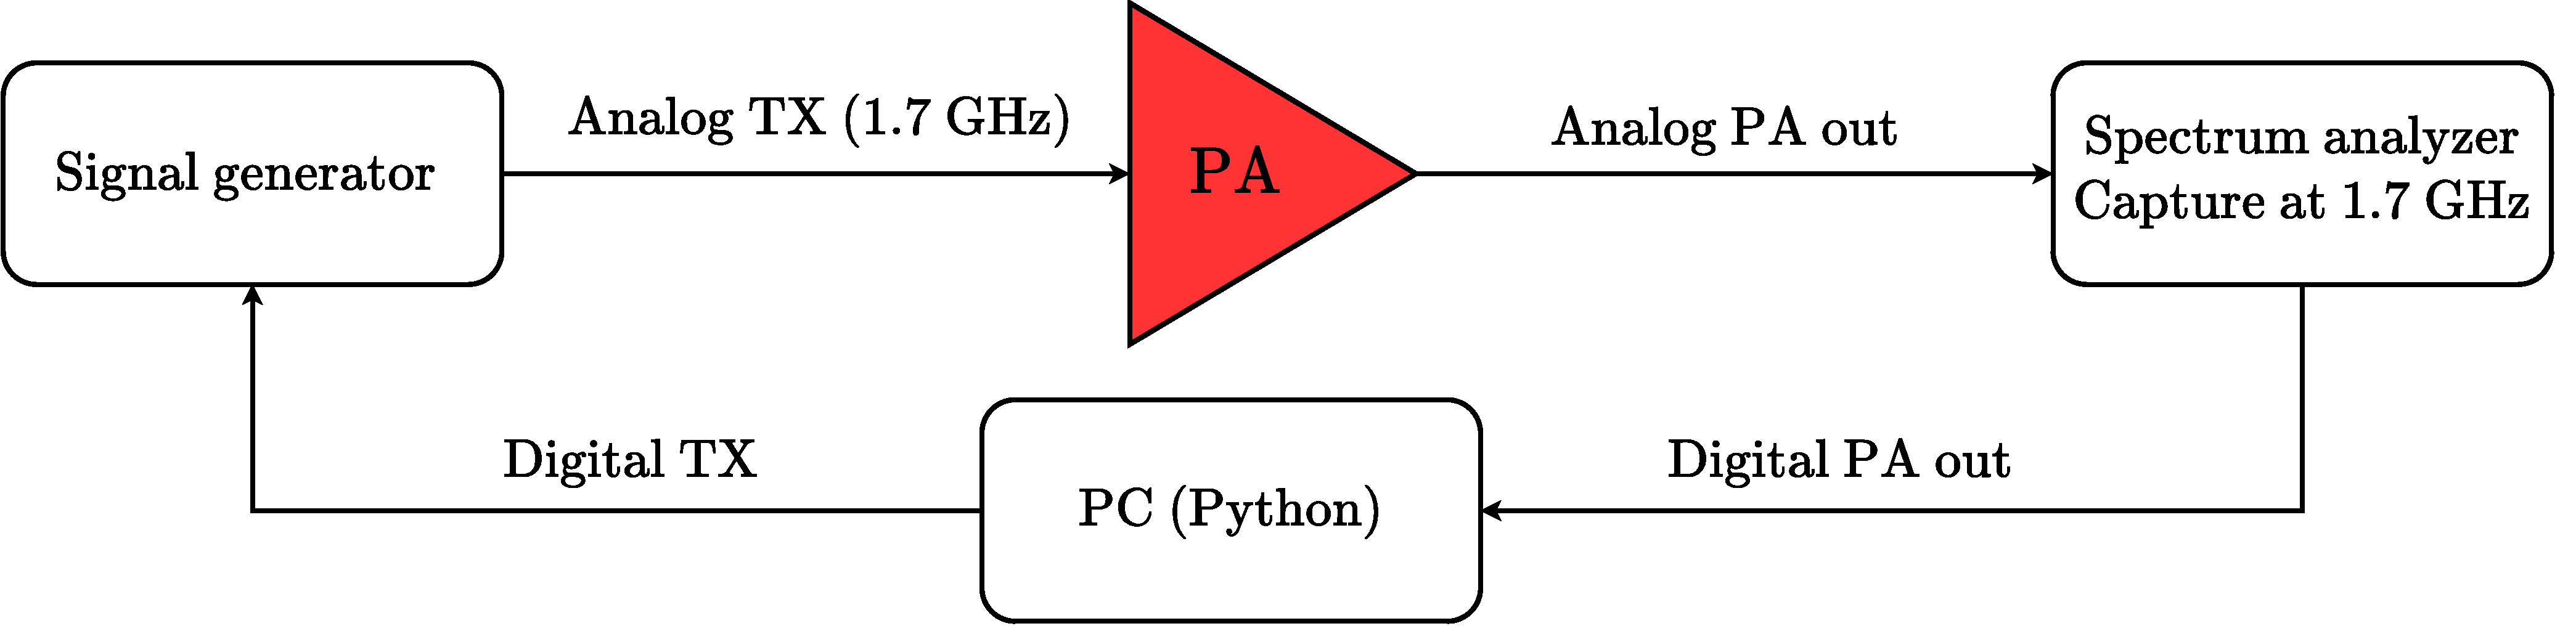
\includegraphics[scale=0.15]{../figures/install/install.pdf}
		\caption{Testbench \{Degtyarev A., draw.io\}}
	\end{figure}
	\begin{itemize}
		\item TX -- QAM modulated OFDM signal, 60 MHz bandwidth, 480 MHz sample rate
		\item Average PA output power 20 dBm
		\item Leakage path is simulated by digital FIR
		\item Hammerstein model: NL -- polynomial order 8, FIR -- 45 taps
	\end{itemize}
\end{frame}

\subsection{Simulation results}
\begin{frame}
	\frametitle{Learning curves}
	\begin{figure}
		\subfloat[BGD with Momentum, BGD with Adam and MNM learning curves on train and test data sets]{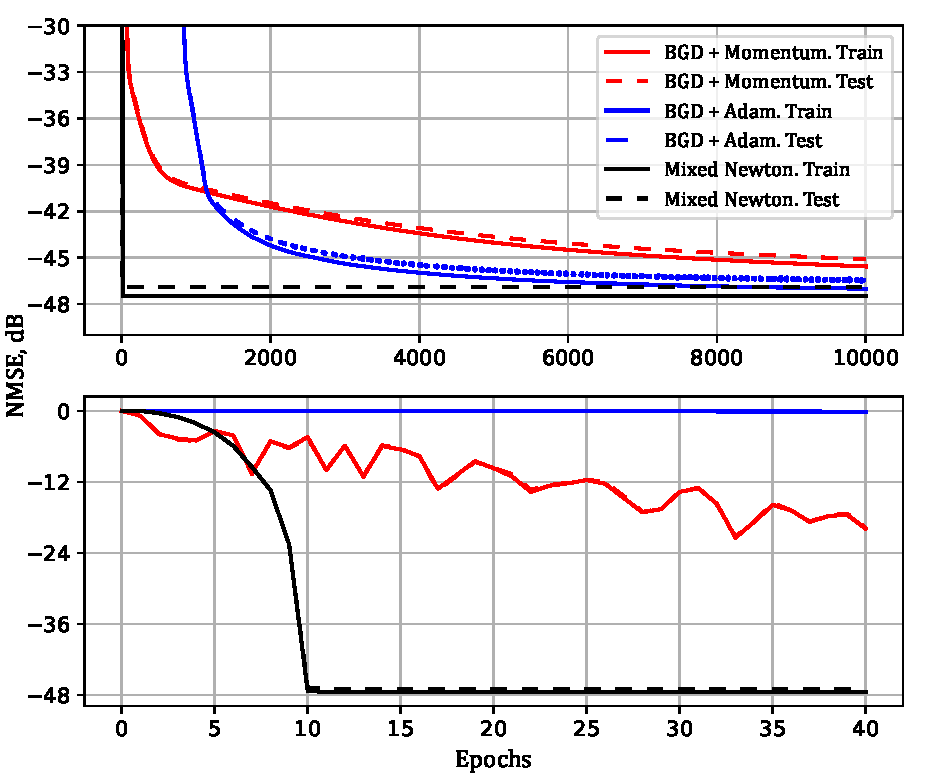
\includegraphics[scale=0.34]{../figures/mnm_bgd/mnm_bgd.pdf}}
		\subfloat[SGD with Momentum, SGD with Adam and MNM learning curves on train and test data sets]{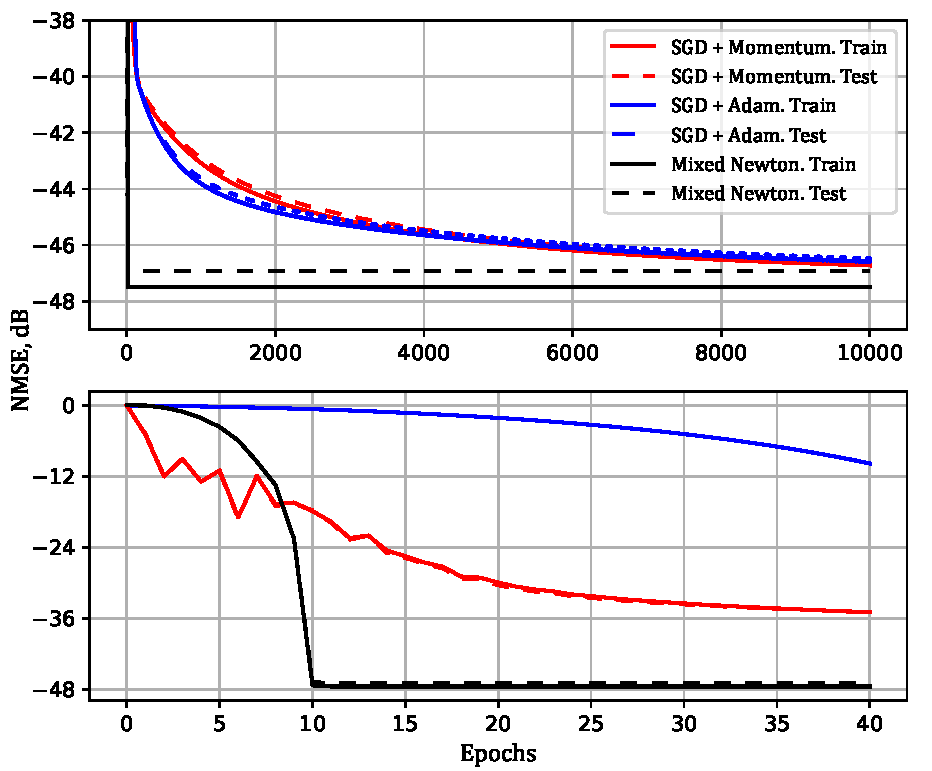
\includegraphics[scale=0.34]{../figures/mnm_sgd/mnm_sgd.pdf}}
	\end{figure}
	\begin{itemize}
		\item Mixed Newton achieves final performance in $\sim$30 epochs, comparing to gradient-based methods ($\sim$10000 epochs)
	\end{itemize}
\end{frame}

\begin{frame}
	\frametitle{Algorithm performance}
	\begin{figure}[htbp]
		\centering
		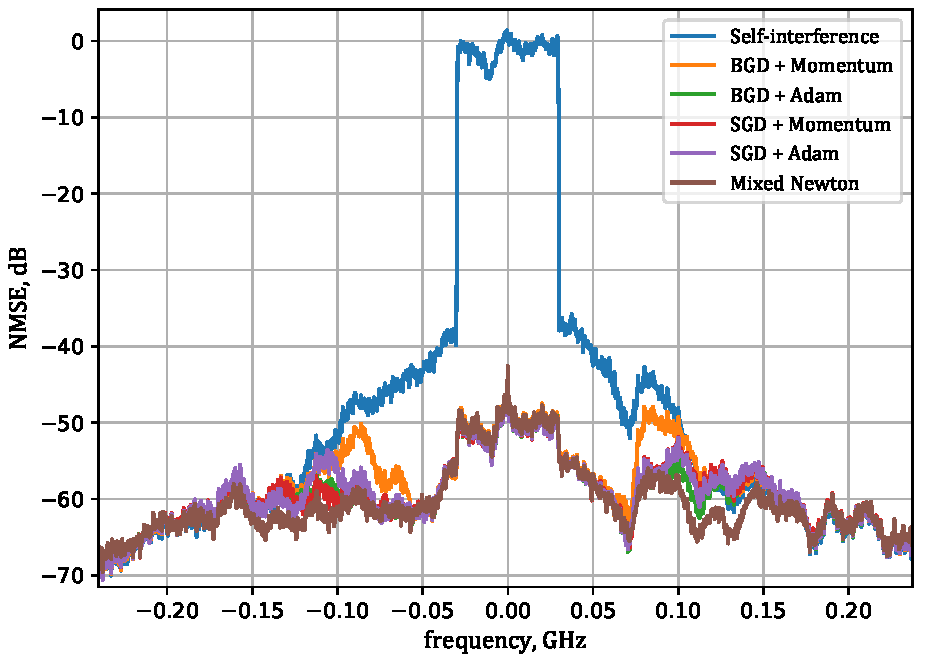
\includegraphics[scale=0.55]{../figures/psd/psd.pdf}
		\centering
		\caption{Power spectral densities of initial and suppressed interference. Signal power distribution along the frequency \{Degtyarev A., Python\}}
	\end{figure}
\end{frame}

\begin{frame}
	\frametitle{Convergence speed comparison}
	\begin{table}[h!]
		\centering
		\caption{Performance and convergence speed comparison}
		\begin{tabular}{|l|c|c|c|c|c|}
			\hline
			\textbf{Algorithm} &
			\textbf{\begin{tabular}[c]{@{}c@{}}BGD\\ Moment.\end{tabular}} &
			\textbf{\begin{tabular}[c]{@{}c@{}}BGD\\ Adam\end{tabular}} &
			\textbf{\begin{tabular}[c]{@{}c@{}}SGD \\ Moment.\end{tabular}} &
			\textbf{\begin{tabular}[c]{@{}c@{}}SGD \\ Adam\end{tabular}} &
			\textbf{MNM} \\ \hline
			\textbf{\begin{tabular}[c]{@{}l@{}}Epoch\\ number\end{tabular}} &
			{\color[HTML]{000000} 10000} &
			{\color[HTML]{000000} 10000} &
			{\color[HTML]{000000} 10000} &
			10000 &
			30 \\ \hline
			\textbf{\begin{tabular}[c]{@{}l@{}}Time per\\ epoch, $10^{-2}$ s\end{tabular}} &
			{\color[HTML]{000000} 3.8} &
			{\color[HTML]{000000} 4.0} &
			{\color[HTML]{000000} 3.7} &
			4.1 &
			21 \\ \hline
			\textbf{\begin{tabular}[c]{@{}l@{}}Total elapsed\\ tims, s\end{tabular}} &
			{\color[HTML]{000000} 380} &
			{\color[HTML]{000000} 403} &
			{\color[HTML]{000000} 386} &
			412 &
			6.2 \\ \hline
			\multirow{2}{*}{\textbf{NMSE, dB}} &
			\multirow{2}{*}{-45.1} &
			\multirow{2}{*}{-46.7} &
			\multirow{2}{*}{-46.6} &
			\multirow{2}{*}{-46.5} &
			\multirow{2}{*}{-46.9} \\ 
			& & & & & \\ \hline 
		\end{tabular}
		\label{table_of_results}
	\end{table}
	\begin{itemize}
		\item MNM step is $\sim$5 times longer comparing to gradient  methods
		\item Total convergence time decreased significantly 
	\end{itemize}
\end{frame}

\section{Conclusions and further work}
\begin{frame}
\frametitle{Conclusions and further work}
\begin{itemize}
\item Total training time is decreased to 6 s comparing to 380 s for gradient-based methods to achieve $\sim$46.5 dB suppression
\item Mixed Newton requires high memory and computation resources due to hessian calculation and inversion
\item Mixed Newton can be modified by inverse hessian (or diagonal) estimation to reduce required resources
\item Application of modified version to complex-valued NN structures

\end{itemize}
\end{frame}
\end{document}